\chapter{Total Synthesis: Strategy and Classic Routes}\label{ch:b3:total-synthesis}

The anticancer drug paclitaxel was first isolated from the bark of the Pacific
yew, a slow-growing tree; stripping the bark killed the tree, and the supply was
far short of what patients needed. Chemists answered in two ways: total
syntheses, which showed that the molecule could be built from simple starting
materials but were far too long for production, and a \omterm{def:b3:total-synthesis:total}{semisynthesis} from a
related compound extracted from the needles of a common yew, which is renewable.
This chapter is about how such routes are judged and designed: how yields
multiply, why convergence pays, what protecting groups cost, which bonds to
make first, and three landmark syntheses read with those tools.

\begin{recall}
The Year 2 volume treated retrosynthetic analysis (target molecule,
disconnection, synthon, synthetic equivalent, functional-group
interconversion), orthogonal protecting groups, the aldol reaction, the
Robinson annulation, the Wittig reaction and iminium chemistry; the Year 1
volume protecting groups and yields. \Cref{ch:b3:asymmetric-synthesis},
\cref{ch:b3:pericyclic} and \cref{ch:b3:homogeneous-catalysis} supplied the
modern key steps.
\end{recall}

\begin{omfigure}
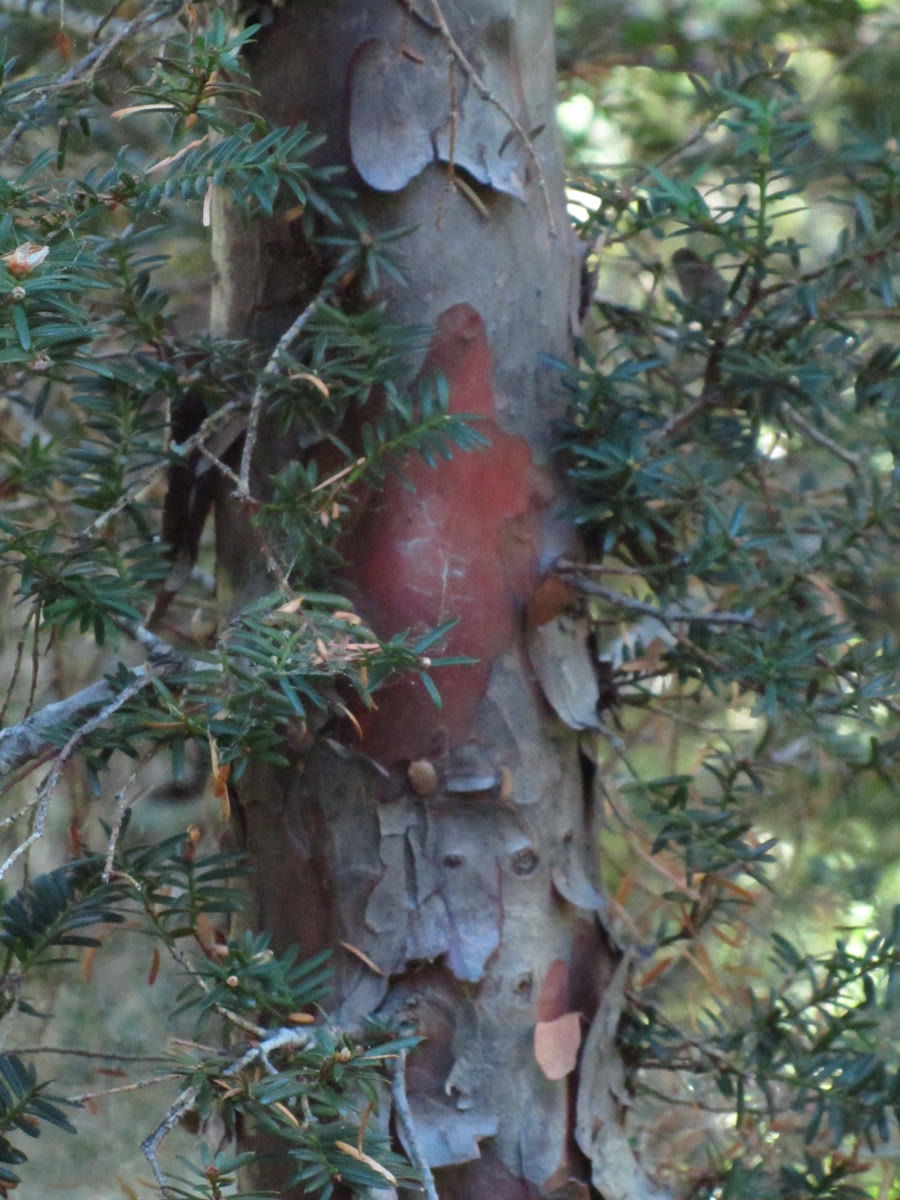
\includegraphics[width=0.32\linewidth]{images/book4/pacific-yew.jpg}

{\small Bark and needles of a Pacific yew, the first source of paclitaxel.
Photograph: JOE BLOWE, CC BY-SA 2.0.}
\end{omfigure}

\section{Measuring a synthesis}

\begin{definition}[Total synthesis]\label{def:b3:total-synthesis:total}
A \emph{total synthesis}\index{total synthesis} makes a complex molecule, often
a natural product, from simple commercial compounds. A \emph{formal
synthesis}\index{formal synthesis} makes an intermediate of an earlier total
synthesis, completing the route on paper. A \emph{semisynthesis}\index{semisynthesis}
starts from a natural compound already close to the target.
\end{definition}

\begin{definition}[Route architecture]\label{def:b3:total-synthesis:architecture}
In a \emph{linear synthesis}\index{linear synthesis} each step acts on the
product of the one before; in a \emph{convergent synthesis}\index{convergent synthesis}
separate fragments are made in parallel and joined late. The
\emph{longest linear sequence}\index{longest linear sequence} (LLS) is the
largest number of steps from any starting material to the target. The
\emph{overall yield}\index{overall yield} is the amount of target obtained
divided by the amount of the limiting starting material.
\end{definition}

\begin{proposition}[Overall yield]\label{prop:b3:total-synthesis:overall-yield}
For a sequence of steps of yields $y_1, \dots, y_n$, the \omterm{def:b3:total-synthesis:architecture}{overall yield} is $Y = \prod_i y_i$.
\end{proposition}

\begin{proof}
Each step converts the amount it receives into $y_i$ times as much product; the
amount reaching the target is the starting amount multiplied by every factor in
turn.
\end{proof}

\begin{proposition}[Convergence]\label{prop:b3:total-synthesis:convergent}
A route of $n = 2m + 1$ steps of equal yield $y$, built as two branches of $m$ steps joined by
one coupling step, has the \omterm{def:b3:total-synthesis:architecture}{overall yield} $y^{m+1}$ along its \omterm{def:b3:total-synthesis:architecture}{longest linear sequence},
against $y^{2m+1}$ for the linear route of the same steps.
\end{proposition}

\begin{proof}
Each branch is made separately, on as much starting material as needed: the
material of each branch passes through $m$ steps and then the coupling, $m + 1$
factors $y$. In the linear route the material passes through all $2m + 1$. For $m = 10$
and $y = 0.90$: 31\,\% against 11\,\%.
\end{proof}

\begin{omfigure}
\begin{tikzpicture}
\begin{axis}[width=0.7\linewidth, height=5.8cm, xmin=0, xmax=30, ymin=0, ymax=1.02,
  axis lines=left, xlabel={number of steps $n$}, ylabel={overall yield},
  tick label style={font=\scriptsize}, label style={font=\small},
  legend style={font=\scriptsize, draw=none, at={(1.03,0.5)}, anchor=west}, legend cell align=left]
\addplot[color=omDef, thick] table[x=n, y=y95] {figdata/out/bachelor-3-overall-yield.dat};
\addlegendentry{95\,\% per step}
\addplot[color=omMeth, thick] table[x=n, y=y90] {figdata/out/bachelor-3-overall-yield.dat};
\addlegendentry{90\,\%}
\addplot[color=omThm, thick] table[x=n, y=y80] {figdata/out/bachelor-3-overall-yield.dat};
\addlegendentry{80\,\%}
\addplot[color=omMeth, thick, dashed, mark=*, mark size=1pt] table[x=n, y=y90] {figdata/out/bachelor-3-overall-yield-b.dat};
\addlegendentry{90\,\%, convergent}
\end{axis}
\end{tikzpicture}

{\small \omterm{def:b3:total-synthesis:architecture}{Overall yield} against the number of steps for three yields per step
(solid: linear routes), and for convergent routes at 90\,\% per step (two equal
branches joined in a last step; dashed). Twenty steps at 90\,\% leave 12\,\%; the
same steps arranged convergently leave about three times more.}
\end{omfigure}

\begin{omfigure}
\begin{tikzpicture}[font=\scriptsize, >=Stealth, node distance=0.9cm,
  st/.style={circle, draw, fill=omDef!15, minimum size=4mm, inner sep=0pt}]
  \foreach \i in {0,...,6} { \node[st] (l\i) at (\i*0.9,1.6) {}; }
  \foreach \i in {0,...,5} { \pgfmathtruncatemacro\j{\i+1} \draw[->] (l\i) -- (l\j); }
  \node[anchor=west] at (6.0,1.6) {linear: 6 steps, LLS 6};
  \foreach \i in {0,...,2} { \node[st] (a\i) at (\i*0.9,0.6) {}; \node[st] (b\i) at (\i*0.9,-0.6) {}; }
  \draw[->] (a0) -- (a1); \draw[->] (a1) -- (a2); \draw[->] (b0) -- (b1); \draw[->] (b1) -- (b2);
  \node[st, fill=omThm!25] (t) at (3.0,0) {};
  \draw[->] (a2) -- (t); \draw[->] (b2) -- (t);
  \node[anchor=west] at (3.4,0) {convergent: 5 steps, LLS 3};
\end{tikzpicture}

{\small Route trees: each circle is a compound, each arrow a step. A linear route
passes all its material through every step; a convergent one makes two fragments
side by side and couples them, so that its \omterm{def:b3:total-synthesis:architecture}{longest linear sequence} is shorter.}
\end{omfigure}

\begin{definition}[Economies and ideality]\label{def:b3:total-synthesis:economy}
\emph{Step economy}\index{step economy} is the aim of reaching a target in as
few steps as possible; \emph{protecting-group economy}\index{protecting-group economy},
that of using as few protection and deprotection steps as possible. The
\emph{ideality}\index{ideality} of a route is the fraction of its steps that
build the skeleton or make a necessary change of oxidation level:
$(\text{construction steps} + \text{strategic redox steps})/(\text{total steps})$.
\end{definition}

\begin{proposition}[Ideality of a route]\label{prop:b3:total-synthesis:ideality}
A one-pot route that only forms skeletal bonds has \omterm{def:b3:total-synthesis:economy}{ideality} 100\,\%; each protection,
deprotection, functional-group interconversion or non-strategic redox step
lowers it.
\end{proposition}

\begin{proof}
Directly from the definition: such steps add to the denominator without adding
to the numerator.
\end{proof}

\section{Protecting groups and their economy}

Each protecting group costs at least two steps, the reagents to put it on and
take it off, and the material lost in both. A route of eight steps at 90\,\% keeps
43\,\% of its material; adding two protections and two deprotections at 95\,\% each
brings it to 35\,\%. Protecting groups are chosen orthogonal, so that each can be
removed without touching the others; better still, the order of steps is
arranged so that the reactive group is not present, or not yet revealed, when
it would interfere: protecting-group-free syntheses are a goal, not a curiosity.

\begin{method}[Reading a total synthesis]\label{met:b3:total-synthesis:analyse}
\begin{enumerate}
  \item Identify the target's rings, stereocentres and sensitive groups.
  \item Find the key disconnections and the reactions that make them in the forward
        direction (\omterm{def:b3:total-synthesis:strategic-bond}{strategic bonds}).
  \item Count the steps and find the \omterm{def:b3:total-synthesis:architecture}{longest linear sequence}; note the convergence.
  \item Note how each stereocentre is set (substrate control, auxiliary, catalyst,
        \omterm{def:b3:asymmetric-synthesis:chiral-pool}{chiral pool}).
  \item List the protecting groups and other non-ideal steps; compute the \omterm{def:b3:total-synthesis:architecture}{overall
        yield} and the \omterm{def:b3:total-synthesis:economy}{ideality}.
\end{enumerate}
\end{method}

\begin{method}[Counting steps]\label{met:b3:total-synthesis:count}
\begin{enumerate}
  \item A step is one operation ending in an isolated (or at least worked-up)
        product; a one-pot sequence without isolation counts as one step.
  \item Count all steps for the total; for the LLS, follow the longest path from a
        commercial compound to the target.
  \item Multiply the yields along the LLS for the \omterm{def:b3:total-synthesis:architecture}{overall yield}.
\end{enumerate}
\end{method}

\section{Strategic bonds and key ring-forming steps}

\begin{definition}[Strategic bond]\label{def:b3:total-synthesis:strategic-bond}
A \emph{strategic bond} of a target\index{strategic bond} is a bond whose
disconnection simplifies the target most, usually by splitting a ring system
or removing several stereocentres at once, and which a reliable reaction can
form.
\end{definition}

Ring-forming reactions that make two bonds or several stereocentres at once
are the workhorses: the Diels--Alder reaction (two C--C bonds, up to four
stereocentres, stereospecifically, \cref{ch:b3:pericyclic}), the Robinson
annulation (a six-membered ring onto a ketone), \omterm{def:b3:homogeneous-catalysis:metathesis}{ring-closing metathesis}
(\cref{ch:b3:homogeneous-catalysis}) for medium and large rings, and cascades.

\begin{definition}[Cascade reaction]\label{def:b3:total-synthesis:cascade}
A \emph{cascade reaction}\index{cascade reaction} is a sequence of
transformations in which each step creates the functionality for the next,
without isolating intermediates or adding reagents.
\end{definition}

\begin{definition}[Biomimetic synthesis]\label{def:b3:total-synthesis:biomimetic}
A \emph{biomimetic synthesis}\index{biomimetic synthesis} imitates the route
by which a natural product is thought to be made in the organism.
\end{definition}

The cyclisation of squalene oxide to lanosterol in cells, four rings and seven
stereocentres in one enzymatic cascade, inspired the polyene cyclisations of
William Johnson, in which a cation started at one end of a carefully designed
polyene closes ring after ring through chair-like transition states, setting
the \textit{trans} ring fusions of the steroids.

\section{Landmark routes}

\begin{definition}[Mannich reaction]\label{def:b3:total-synthesis:mannich}
The \emph{Mannich reaction}\index{Mannich reaction} is the addition of an enol
or enolate to an iminium ion, made in situ from an aldehyde and a primary or
secondary amine, giving a $\beta$-amino carbonyl compound.
\end{definition}

In 1917 Robert Robinson made tropinone, the bicyclic core of atropine and
cocaine, in one pot from three simple components in water, imagining that the
plant might build it the same way:
$\ce{C4H6O2 + CH3NH2 + C5H6O5 -> C8H13NO + 2CO2 + 2H2O}$ (succinaldehyde, methylamine and
acetonedicarboxylic acid give tropinone).

\begin{omfigure}
\begin{tikzpicture}[font=\small, >=Stealth]
  \node[align=center] at (-0.5,0) {$\ce{OHC-CH2CH2-CHO}$\\ $+\ \ce{CH3NH2}$\\ $+\ \ce{HO2C-CH2-CO-CH2-CO2H}$};
  \draw[->, thick] (3.0,0) -- (4.7,0) node[midway, above, font=\scriptsize] {buffered water} node[midway, below, font=\scriptsize] {$-\ce{2CO2}$, $-\ce{2H2O}$};
  \begin{scope}[xshift=6.1cm, yshift=-0.2cm]
    \coordinate (c1) at (-1,0.3); \coordinate (c2) at (-0.8,-0.5); \coordinate (c3) at (0,-0.9);
    \coordinate (c4) at (0.8,-0.5); \coordinate (c5) at (1,0.3); \coordinate (c6) at (0.45,1.15);
    \coordinate (c7) at (-0.45,1.15); \coordinate (n) at (0,0.45);
    \draw[thick] (c1) -- (c2) -- (c3) -- (c4) -- (c5) -- (c6);
    \draw[thick] (c7) -- (c1);
    \draw[thick] (c6) -- (0.12,1.15); \draw[thick] (-0.12,1.15) -- (c7);
    \draw[thick] (c1) -- (n) -- (c5);
    \draw[thick] (n) -- (0,1.6) node[above, inner sep=1pt] {$\ce{CH3}$};
    \draw[thick, double, double distance=1.5pt] (c3) -- (0,-1.55) node[below, inner sep=1pt] {O};
    \node[fill=white, inner sep=0.5pt] at (n) {N};
    \node[font=\scriptsize, anchor=west] at (1.2,0.3) {tropinone};
  \end{scope}
\end{tikzpicture}

{\small Robinson's tropinone synthesis. Two \omterm{def:b3:total-synthesis:mannich}{Mannich reactions}, the first
intermolecular and the second closing the ring, join the three components;
the two carboxylic acid groups that made the central $\ce{CH2}$ groups enolisable then
leave as carbon dioxide. In the bicyclic product the N-methyl bridge spans the
seven-membered ring.}
\end{omfigure}

\begin{proposition}[Tropinone in one pot]\label{prop:b3:total-synthesis:tropinone}
The one-pot tropinone synthesis is two \omterm{def:b3:total-synthesis:mannich}{Mannich reactions} followed by two
decarboxylations.
\end{proposition}

\begin{proof}[Argued]
Methylamine and one aldehyde group of succinaldehyde give an iminium ion; an
enol of acetonedicarboxylic acid adds to it (first Mannich). The secondary
amine formed condenses with the second aldehyde group into a cyclic iminium
ion, which the enol on the other side of the ketone attacks (second Mannich),
closing the bicycle. The two $\beta$-keto acid groups then lose $\ce{CO2}$, as $\beta$-keto acids do
on mild warming.
\end{proof}

Elias Corey's synthesis of prostaglandin $\mathrm F_{2\alpha}$ (1969) made retrosynthetic analysis
explicit. A bicyclo[2.2.1]heptenone built by a Diels--Alder reaction carries
the relative configuration of the cyclopentane's substituents; a
\omterm{def:b3:radicals-carbenes:baeyer}{Baeyer--Villiger oxidation} (\cref{ch:b3:radicals-carbenes}) and an
iodolactonisation turn it into the Corey lactone, from which the two side chains
are attached by olefinations. The lactone has served for many prostaglandin
drugs since.

\begin{omfigure}
\begin{tikzpicture}[font=\small,
  box/.style={draw, rounded corners, align=center, fill=omDef!8, inner sep=4pt}]
  \node[box] (t) at (0,0) {prostaglandin\\ $\mathrm F_{2\alpha}$};
  \node[box] (l) at (4.4,0) {Corey lactone\\ (four\\ stereocentres)};
  \node[box] (b) at (9.2,0) {bicyclo[2.2.1]-\\ heptenone};
  \node[box] (d) at (9.2,-2.4) {substituted\\ cyclopentadiene $+$\\ ketene equivalent};
  \draw[omretro] (t) -- (l) node[midway, above=3pt, font=\scriptsize] {olefinations};
  \draw[omretro] (l) -- (b) node[midway, above=3pt, font=\scriptsize, align=center] {iodolactonisation,\\ Baeyer--Villiger};
  \draw[omretro] (b) -- (d) node[midway, right, font=\scriptsize] {Diels--Alder};
\end{tikzpicture}

{\small Corey's retrosynthesis of prostaglandin $\mathrm F_{2\alpha}$, in outline (double arrows: ``is
made from''). The two side chains are disconnected first; the cyclopentane with
its four stereocentres comes from a lactone, the lactone from a bicyclic ketone,
and the ketone from a Diels--Alder reaction that sets their relative
configuration.}
\end{omfigure}

Oseltamivir, the influenza drug, is made industrially from shikimic acid, a
chiral-pool compound extracted from star anise and later produced by
fermentation: its six-membered ring and stereocentres are already in place.
The route converts the ring diol into an epoxide, opens it with azide, closes an
aziridine and opens that with azide again, setting the two nitrogen atoms
\textit{trans}; acetylation and reduction finish the job. Because sodium azide and
organic azides are toxic and potentially explosive on a large scale, azide-free
routes were later developed.

\begin{omfigure}
\begin{tikzpicture}[font=\scriptsize, >=Stealth,
  box/.style={draw, rounded corners, align=center, fill=omMeth!8, inner sep=3pt}]
  \node[box] (a) at (0,0) {($-$)-shikimic acid\\ (chiral pool)};
  \node[box] (b) at (3.1,0) {ester, ketal,\\ mesylate};
  \node[box] (c) at (6.0,0) {epoxide};
  \node[box] (d) at (8.6,0) {azido alcohol};
  \node[box] (e) at (8.6,-1.5) {aziridine};
  \node[box] (f) at (5.4,-1.5) {\textit{trans}-diamine\\ precursor (azide)};
  \node[box] (g) at (1.6,-1.5) {oseltamivir\\ phosphate};
  \draw[->] (a) -- (b); \draw[->] (b) -- (c); \draw[->] (c) -- (d) node[midway, above] {$\ce{N3-}$};
  \draw[->] (d) -- (e); \draw[->] (e) -- (f) node[midway, above] {$\ce{N3-}$};
  \draw[->] (f) -- (g) node[midway, below, align=center] {acetylation,\\ reduction};
\end{tikzpicture}

{\small Oseltamivir from shikimic acid, key stages only: the natural ring and its
stereocentres are kept, and two nitrogen atoms are introduced \textit{trans} to each other
by successive openings of an epoxide and an aziridine with azide.}
\end{omfigure}

\section{From discovery to process}

A route that delivers milligrams for biological testing is rarely the one used
for tonnes. Process chemists scout routes for cost, safety and robustness:
they remove chromatography in favour of crystallisation, replace hazardous
reagents and cryogenic temperatures, shorten the sequence, check the thermal
safety of every step by calorimetry, and set specifications for impurities.
These choices meet the measures of \cref{ch:b3:green-industrial}.

\begin{inthelab}[From one gram to one kilogram]
A step run on one gram in a round-bottomed flask is repeated at ten grams in a
jacketed reactor with an overhead stirrer and a temperature probe in the
liquid, adding the reactive reagent at a controlled rate while watching the
internal temperature: the heat released grows with the volume, but the area that
removes it grows only as the square of the size. Only when the heat flow and the work-up
(phase separations, filtrations, drying) behave is the step run at a kilogram.
\end{inthelab}

\begin{safety}{\ghs[0.62cm]{GHS06}\ghs[0.62cm]{GHS08}\ghs[0.62cm]{GHS09}}
% ledger: ghs4:NaN3
Sodium azide: fatal if swallowed, very toxic to aquatic life; with acids it
releases hydrazoic acid, a toxic and explosive gas, and with heavy metals
(copper and lead in drains) it forms explosive azides. Waste is destroyed
chemically, never poured away.
\end{safety}

\begin{history}[Robinson, Woodward, Corey]
Robert Robinson received the 1947 Nobel Prize in Chemistry for his work on
alkaloids and other plant products; his tropinone synthesis of 1917 is still
quoted for its economy. Robert Woodward's syntheses of quinine, cholesterol,
chlorophyll and, with Albert Eschenmoser, vitamin $\mathrm B_{12}$ made \omterm{def:b3:total-synthesis:total}{total synthesis} an art
(1965 prize). Elias Corey formalised retrosynthetic analysis and received the
1990 prize for the theory and methodology of organic synthesis.
\end{history}

\section{Exercises}

\begin{exercise}[$\star$]\label{exo:b3:total-synthesis:1}
Compute the \omterm{def:b3:total-synthesis:architecture}{overall yield} of 10- and 20-step linear routes at 90\,\% and at 80\,\% per
step.
\end{exercise}

\begin{exercise}[$\star$]\label{exo:b3:total-synthesis:2}
A route makes fragment A in five steps and fragment B in three, couples them, and
needs four more steps to the target. Give the total number of steps and the
\omterm{def:b3:total-synthesis:architecture}{longest linear sequence}.
\end{exercise}

\begin{exercise}[$\star$]\label{exo:b3:total-synthesis:3}
Give the product of the \omterm{def:b3:total-synthesis:mannich}{Mannich reaction} of acetone, formaldehyde and
dimethylamine.
\end{exercise}

\begin{exercise}[$\star$]\label{exo:b3:total-synthesis:4}
Give a Diels--Alder disconnection of 4-acetylcyclohexene, and the forward
reaction.
\end{exercise}

\begin{exercise}[$\star\star$]\label{exo:b3:total-synthesis:5}
A 21-step linear route runs at 90\,\% per step. Compute its \omterm{def:b3:total-synthesis:architecture}{overall yield} and that
of a convergent version with two 10-step branches and one coupling.
\end{exercise}

\begin{exercise}[$\star\star$]\label{exo:b3:total-synthesis:6}
Route A has 12 steps, of which 7 make skeletal bonds and 1 is a strategic
reduction; route B has 9 steps, 7 of them skeletal. Compute their idealities.
\end{exercise}

\begin{exercise}[$\star\star$]\label{exo:b3:total-synthesis:7}
An eight-step route at 90\,\% per step needs two protecting groups, each put on and
taken off at 95\,\%. Compute the \omterm{def:b3:total-synthesis:architecture}{overall yield} with and without them.
\end{exercise}

\begin{exercise}[$\star\star$]\label{exo:b3:total-synthesis:8}
A triol has a primary, a secondary and a tertiary hydroxy group. Propose
protecting groups that allow each to be revealed in turn, and their removal
conditions.
\end{exercise}

\begin{exercise}[$\star\star$]\label{exo:b3:total-synthesis:9}
Why was paclitaxel produced by \omterm{def:b3:total-synthesis:total}{semisynthesis} rather than by any of its total
syntheses?
\end{exercise}

\begin{exercise}[$\star\star\star$]\label{exo:b3:total-synthesis:10}
2-Methylcyclohexane-1,3-dione reacts with methyl vinyl ketone in a Robinson
annulation. Identify the Michael and aldol steps and give the bicyclic enone
formed (the Wieland--Miescher ketone).
\end{exercise}

\begin{exercise}[$\star\star\star$]\label{exo:b3:total-synthesis:11}
Show that the convergent route of \cref{prop:b3:total-synthesis:convergent} keeps
$y^{-m}$ times more material than the linear one, and evaluate this factor for $m = 5$ and
$m = 15$ at 90\,\%.
\end{exercise}

\begin{exercise}[$\star\star\star$]\label{exo:b3:total-synthesis:12}
In a polyene cyclisation, why do chair-like transition states give \textit{trans} ring
fusions, and why does the geometry (\textit{E} or \textit{Z}) of each double bond matter?
\end{exercise}

\section{Problem: Tropinone in One Pot}

\begin{problem}[{Weekend problem --- tropinone in one pot: the three components
and the balanced equation, the two Mannich reactions, a comparison with a long
linear route, and the stereochemistry of tropinone and its reduction products}]
\label{pb:b3:total-synthesis:1}
% ledger: aw:C, aw:H, aw:N, aw:O
Data of the problem: the one-pot synthesis, run in buffered water near pH 5,
gives tropinone in 42\,\% yield; an older linear route needs 14 steps averaging 75\,\%.

\medskip\noindent\textbf{Part I --- Components and equation.}
\begin{enumerate}
  \item Give the formulas of succinaldehyde, methylamine, acetonedicarboxylic acid
        and tropinone.
  \item Write the balanced equation.
  \item Compute the molar masses of the reactants and of tropinone.
  \item Compute the atom economy.
  \item Why is acetonedicarboxylic acid used instead of acetone?
  \item Why does buffering near neutral pH help?
\end{enumerate}

\medskip\noindent\textbf{Part II --- Mechanism.}
\begin{enumerate}[resume]
  \item Write the formation of the first iminium ion.
  \item Show the first \omterm{def:b3:total-synthesis:mannich}{Mannich reaction}.
  \item How does the second iminium ion form?
  \item Show the second, ring-closing \omterm{def:b3:total-synthesis:mannich}{Mannich reaction}.
  \item Why do the two carboxylic acid groups leave as $\ce{CO2}$?
  \item Count the C--C and C--N bonds formed.
\end{enumerate}

\medskip\noindent\textbf{Part III --- One pot against fourteen steps.}
\begin{enumerate}[resume]
  \item Compute the \omterm{def:b3:total-synthesis:architecture}{overall yield} of the linear route.
  \item Compute the ratio of the one-pot yield to it.
  \item Compute the \omterm{def:b3:total-synthesis:economy}{ideality} of the one-pot route.
  \item What else besides yield favours the one-pot route?
  \item Why is the one-pot synthesis called biomimetic?
  \item Name another reaction class of this chapter that makes several bonds at once.
\end{enumerate}

\medskip\noindent\textbf{Part IV --- Stereochemistry.}
\begin{enumerate}[resume]
  \item Is tropinone chiral? Find its \omterm{def:b3:point-groups:operation}{symmetry element}.
  \item Why are the two bridgehead carbons stereocentres nonetheless?
  \item Reduction of the ketone gives two alcohols, tropine and pseudotropine. What
        is their relationship?
  \item Are tropine and pseudotropine chiral?
  \item Why does a hydride approach the carbonyl group preferentially from one face?
  \item State the result: the ratio of the one-pot yield to the linear route's
        \omterm{def:b3:total-synthesis:architecture}{overall yield}.
\end{enumerate}
\end{problem}
